\section{Modelo conceptual}
\section{Modelo conceptual de casos de uso}

\subsection{Descripción general}
 En la figura~\ref{fig:conceptualProyectos} se muestra la estructura de información que manejará el sistema para registrar proyectos así como la estructura general de los elementos que componen un caso de uso.
 
\begin{figure}[htbp!]
	\begin{center}
		\fbox{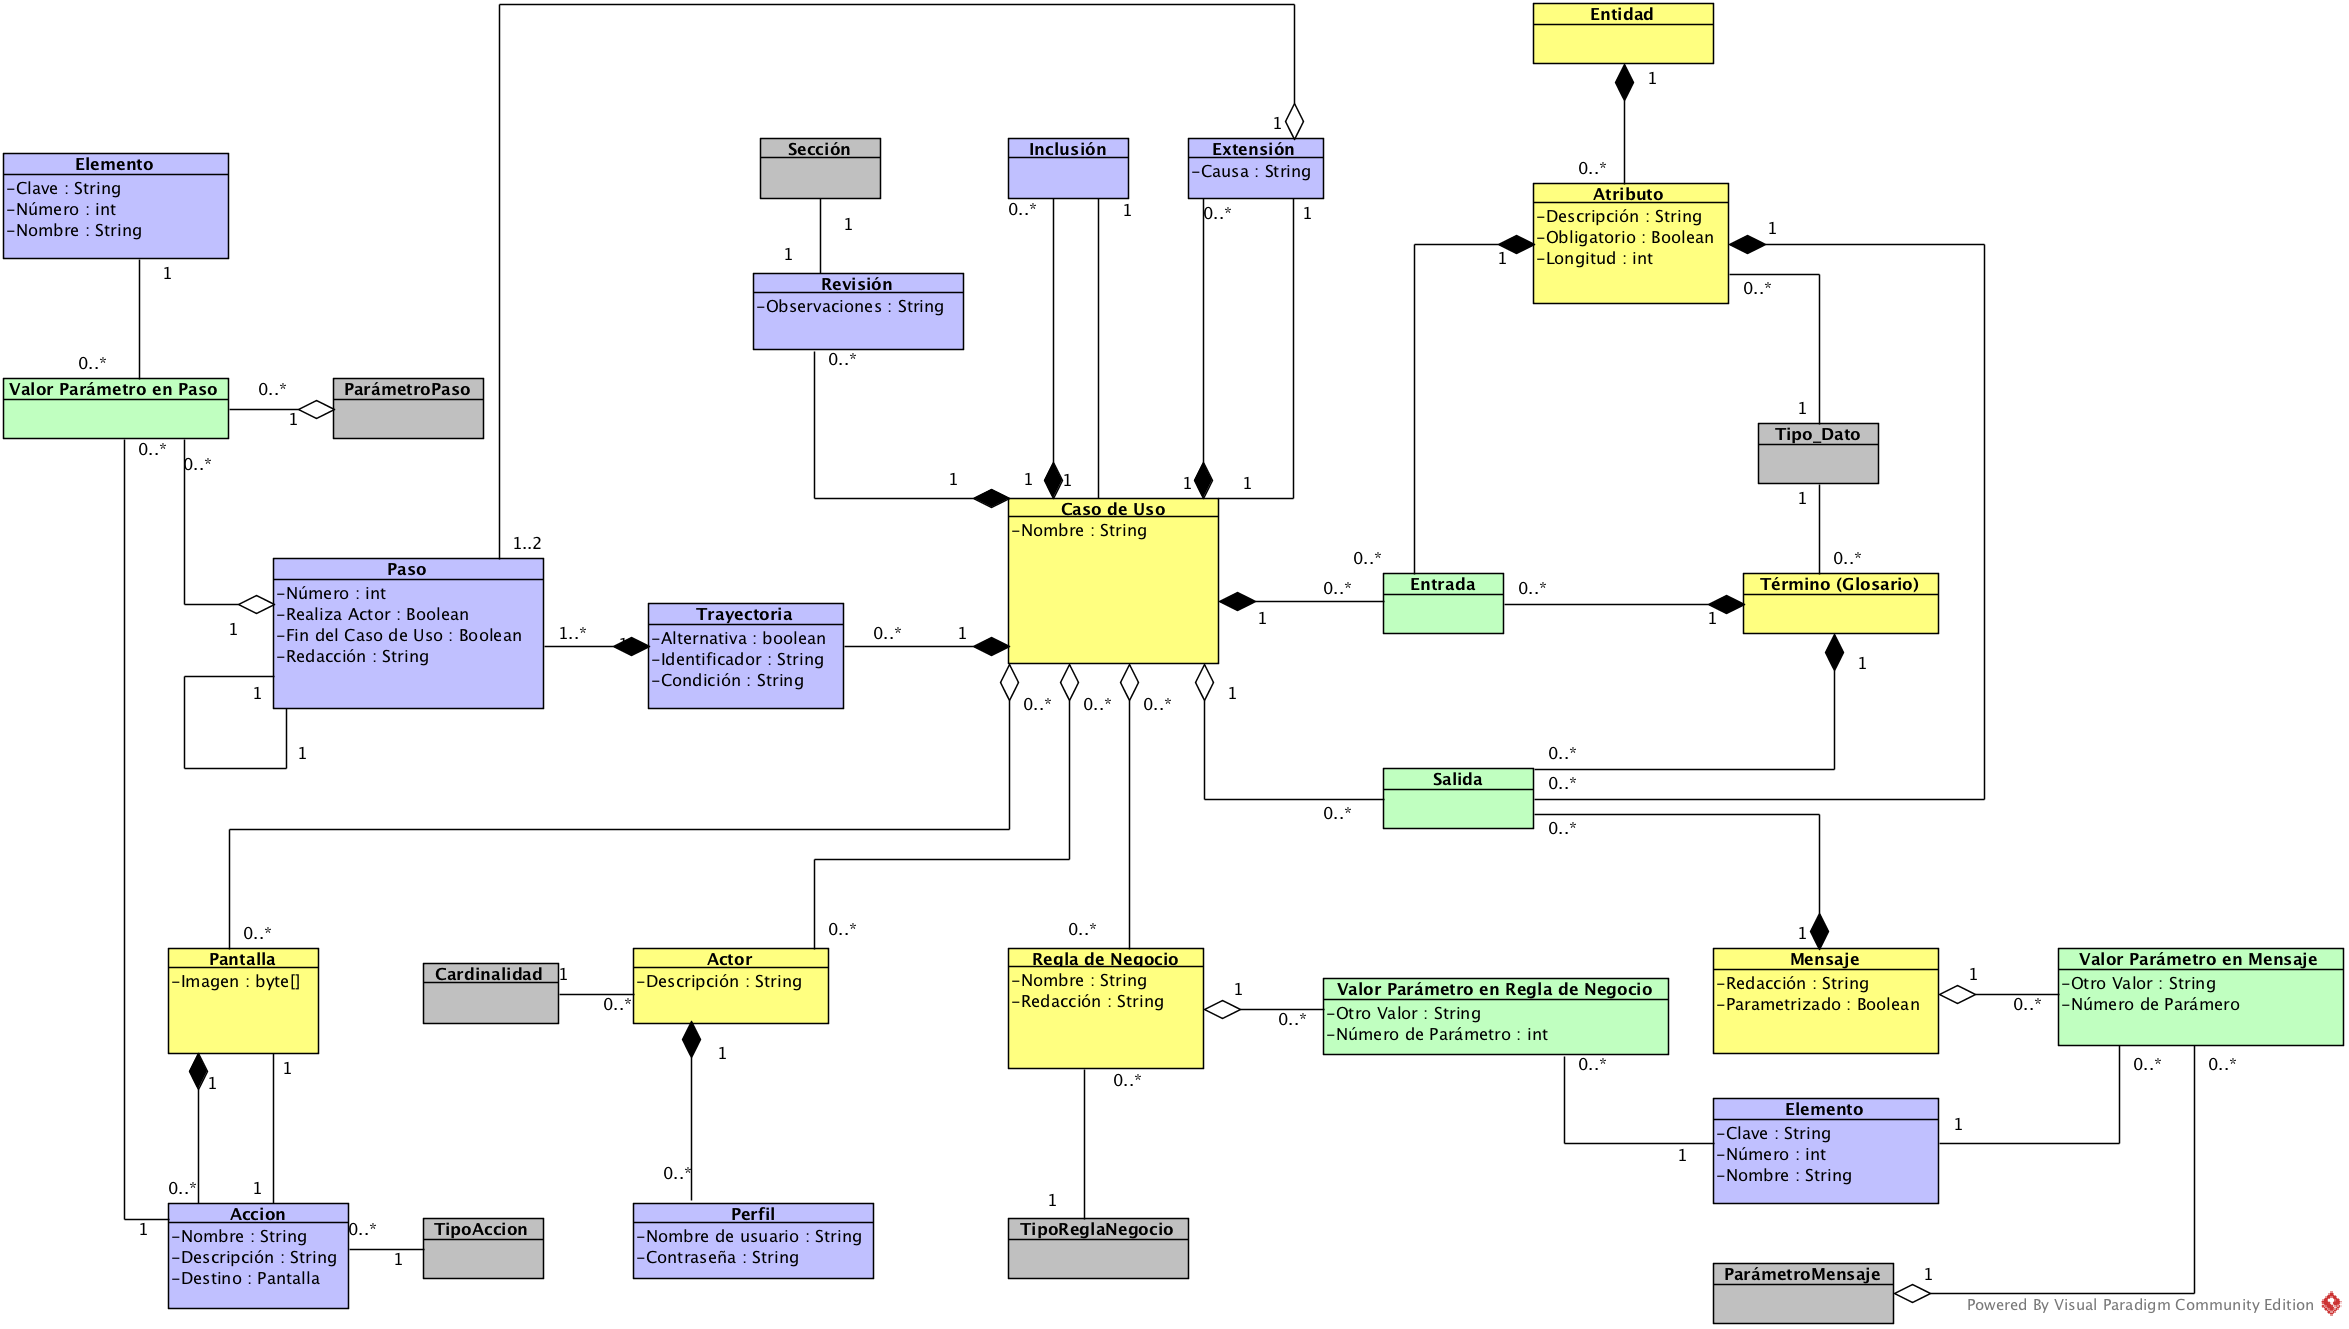
\includegraphics[width=.6\textwidth]{ModeloNegocios/images/ModeloConceptualCasoUso}}
		\caption{Modelo conceptual de proyectos}
		\label{fig:conceptualProyectos}
	\end{center}
\end{figure}

%-----------------------------------------------------------------------------------
\begin{BusinessEntity}{Elemento}{Elemento}
      \Battr{Clave}{Clave}{\tdPalabra}{Clave que permitirá distinguir el tipo de elemento}{\requerido}
      \Battr{Numero}{Número}{\tdNumerico{entero}}{Número del elemento del tipo definido por la Clave}{\requerido}
      \Battr{Nombre}{Nombre}{\tdFrase}{Nombre que identificará al elemento}{\requerido}
\end{BusinessEntity}

\subsubsection{Relaciones}

\begin{BusinessFact}{Elemento:Pantalla}{Pantalla}
	\BRitem{Descripción}{Pantalla es un tipo de \cdtRef{elemento}{Elemento}}
	\BRitem{Tipo}{\relHerencia}
\end{BusinessFact}

\begin{BusinessFact}{Elemento:RegladeNegocio}{Regla de Negocio}
	\BRitem{Descripción}{Regla de Negocio es un tipo de \cdtRef{elemento}{Elemento}}
	\BRitem{Tipo}{\relHerencia}
\end{BusinessFact}

\begin{BusinessFact}{Elemento:Actor}{Actor}
	\BRitem{Descripción}{Actor es un tipo de \cdtRef{elemento}{Elemento}}
	\BRitem{Tipo}{\relHerencia}
\end{BusinessFact}

\begin{BusinessFact}{Elemento:Mensaje}{Mensaje}
	\BRitem{Descripción}{Mensaje es un tipo de \cdtRef{elemento}{Elemento}}
	\BRitem{Tipo}{\relHerencia}
\end{BusinessFact}

\begin{BusinessFact}{Elemento:Termino(Glosario)}{Término (Glosario)}
	\BRitem{Descripción}{Término (Glosario) es un tipo de \cdtRef{elemento}{Elemento}}
	\BRitem{Tipo}{\relHerencia}
\end{BusinessFact}

\begin{BusinessFact}{Elemento:Atributo}{Atributo}
	\BRitem{Descripción}{Atributo es un tipo de \cdtRef{elemento}{Elemento}}
	\BRitem{Tipo}{\relHerencia}
\end{BusinessFact}

\begin{BusinessFact}{Elemento:Entidad}{Entidad}
	\BRitem{Descripción}{Entidad es un tipo de \cdtRef{elemento}{Elemento}}
	\BRitem{Tipo}{\relHerencia}
\end{BusinessFact}

\begin{BusinessFact}{Elemento:CasodeUso}{Caso de Uso}
	\BRitem{Descripción}{Caso de Uso es un tipo de \cdtRef{elemento}{Elemento}}
	\BRitem{Tipo}{\relHerencia}
\end{BusinessFact}

\begin{BusinessFact}{Elemento:Actualizacion}{Actualización}
	\BRitem{Descripción}{Un elemento ha pasado por un conjunto de actualizaciones}
      \BRitem{Tipo}{\relComposicion}
      \BRitem{Cardinalidad}{Uno a muchos}
\end{BusinessFact}

\begin{BusinessFact}{Elemento:EstadoElemento}{EstadoElemento}
		\BRitem{Descripción}{Un elemento se encuentra en un estado}
      	\BRitem{Tipo}{\relAsociacion}
      	\BRitem{Cardinalidad}{Muchos a uno}
\end{BusinessFact}

\begin{BusinessFact}{Elemento:Proyecto}{Proyecto}
	\BRitem{Descripción}{Un proyecto se compone de elementos}
      \BRitem{Tipo}{\relComposicion}
      \BRitem{Cardinalidad}{Muchos a uno}
\end{BusinessFact}

\begin{BusinessFact}{Elemento:ValorParametroenPaso}{Valor Parámetro en Paso}
	\BRitem{Descripción}{Un elemento puede ser el valor de algún parámetro en un paso de la trayectoria}
      \BRitem{Tipo}{\relAsociacion}
      \BRitem{Cardinalidad}{Uno a muchos}
\end{BusinessFact}

\begin{BusinessFact}{Elemento:ValorParametroenMensaje}{Valor Parámetro en Mensaje}
	\BRitem{Descripción}{Un elemento puede ser el valor de algún parámetro en un mensaje}
      \BRitem{Tipo}{\relAsociacion}
      \BRitem{Cardinalidad}{Uno a muchos}
\end{BusinessFact}

\begin{BusinessFact}{Elemento:ValorParametroenRegladeNegocio}{Valor Parámetro en Regla de Negocio}
	\BRitem{Descripción}{Un elemento puede ser el valor de algún parámetro en una regla de negocio}
      \BRitem{Tipo}{\relAsociacion}
      \BRitem{Cardinalidad}{Uno a muchos}
\end{BusinessFact}
%-----------------------------------------------------------------------------------

\begin{BusinessEntity}{CasodeUso}{Caso de Uso}
      \Battr{Clave}{Clave}{\tdPalabra}{Clave que permitirá distinguir el tipo de elemento}{\requerido}
      \Battr{Numero}{Número}{\tdNumerico{entero}}{Número del elemento del tipo definido por la Clave}{\requerido}
      \Battr{Nombre}{Nombre}{\tdFrase}{Nombre que identificará al elemento}{\requerido}
\end{BusinessEntity}

\subsubsection{Relaciones}

\begin{BusinessFact}{Elemento:Pantalla}{Pantalla}
	\BRitem{Descripción}{Pantalla es un tipo de \cdtRef{elemento}{Elemento}}
	\BRitem{Tipo}{\relHerencia}
\end{BusinessFact}

